% !TEX root = main.tex


\newpage
\appendix
\section{Cumulative Variance of the Gradients and Quality of Optimization}  \label{appendix:cumulvariance}
The relationship between cumulative second moment of the gradients and quality of optimization has been demonstrated in several works. Since the difference between the second moment and the variance is independent of the sampling distribution $p_t$, the guarantees of our method also translate to guarantees with respect to the cumulative second moments of the gradient estimates. Here we provide two concrete references.

For the following, assume that we would like to minimize a convex objective,
$$
\min_{w\in\W}F(w): = \Expect_{z\sim \D}[f(w;z)]
$$
and we assume that we are able to draw i.i.d. samples from the unknown distribution $\D$.
Thus, given a point $w\in\W$ we are able to design an unbiased estimate for $\nabla F(w)$ by sampling $z\sim\D$ and taking $g: = \nabla f(w;z)$ (clearly,
$
\expval{g\vert w} = \nabla F(w)
$).
Now assume a gradient-based update rule, i.e.,
\begin{align}\label{eq:GDupdate}
w_{t+1} = \Pi_{\W}(w_t -\eta_t g_t),\quad \text{where}~~~\expval{g_t\vert w_t} = \nabla F(w_t)
\end{align}
and $\Pi_\W(u): = \argmin_{w\in\W}\|u-w\|$.
Next we  show that for two very popular gradient based-methods --- AdaGrad and SGD for strongly-convex functions, the performance is directly related to the cumulative second moment of the gradient estimates, $\sumtt \Expect\|g_t\|^2$. The latter is exactly the objective of our online variance reduction method.

The AdaGrad algorithm employs the same rule as in Eq.~\eqref{eq:GDupdate} using
$\eta_t = D/\sqrt{2\sum_{\tau=1}^t \|g_t\|^2}$. The next theorem substantiates its guarantees.
\begin{theorem}[\cite{duchi2011adaptive}] Assume that the diameter of $\W$ is bounded by $D$. Then:

\begin{equation*}
\expval{F\left(  \frac{1}{T} \sum_{t=1}^T  w_t  \right) } - \min_{w\in\W}F(w) \leq \frac{2D}{ T}\sqrt{ \sumtt \Expect\|g_t\|^2}
\end{equation*}
\end{theorem}

The SGD algorithm for $\mu$-strongly-convex objectives employs the same rule as in Eq.~\eqref{eq:GDupdate} using
$\eta_t = \frac{2}{\mu t}$. The next theorem substantiates its guarantees.




\begin{theorem}[\cite{salehi2017}] Assume that $F$ is $\mu$-strongly convex, then:
\begin{equation*}
\expval{F\left(  \frac{2}{T(T+1)} \sum_{t=1}^T t\cdot w_t  \right) } - \min_{w\in\W}F(w) \leq \frac{2}{\mu T(T+1)} \sumtt \Expect\|g_t\|^2
\end{equation*}
\end{theorem}


\section{Proof of Lemma~\ref{lem:MeaningfulRegret}}
\begin{proof}%[Proof of Lemma~\ref{lem:MeaningfulRegret}]
Denote $\ell^2_{1:t}(i) = \sum_{\tau=1}^t \ell_\tau^2(i)$.
Next, we bound the  cumulative  loss per point $i\in[n]$,
 \begin{align} \label{eq:SumeLL}
  \ell_{1:T}^2(i)= \sum_{t=1}^T {\ell_t^2(i)} 
& =  \sum_{t=1}^T {\left(\ell_*(i) + \left(\ell_t(i)-\ell_*(i)\right) \right)^2}   \nonumber\\
&\leq T\cdot \ell_{*}^2(i) + 2\ell_{*}(i)\sum_{t=1}^T|\ell_t(i) - \ell_{*}(i)| + \sum_{t=1}^T(\ell_t(i) - \ell_{*}(i))^2 \nonumber\\
&\leq T\cdot \ell_{*}^2(i) + 2\ell_{*}(i)\sqrt{T\cdot V_T(i)} +V_T(i)  \nonumber\\
&=T\left(\ell_{*}(i) +   \sqrt{\frac{V_T(i)}{T}} \right)^2
\end{align}
where the second line uses $\ell_*(i)\geq 0$ and the third line uses the definition of $V_T(i)$ together with the inequality
$\|u\|_1\leq \sqrt{T}\|u\|_2,\; \forall u\in \reals^T$.

We require the following lemma:
\begin{lemma}\label{lem:OptValue}
Let $a_1,\ldots,a_n\geq0$. Then the following holds,
$$
\min_{p\in\Delta}\sumin\frac{a_i}{p(i)} =\left( \sumin\sqrt{a_i}\right)^2~.
$$
\end{lemma}
The proof of the lemma is analogous to the proof of Lemma \ref{lemma:ftrl-sol}, which is given in the next section. Notice that according to this lemma and using the non-negativity of losses we have,
\begin{align} \label{eq:OptimalPerpoint}
\frac{1}{n^2}\min_{p\in\Delta}\sumin \frac{\ell_t^2(i)}{p(i)} =\left(\frac{1}{n} \sumin \ell_t(i) \right)^2:= L^2(w_t)~.
\end{align}
We are now ready to bound the value of best fixed point in hindsight,
\begin{align*}
\min_{p} \frac{1}{n^2}\sum_{t=1}^T \sumin \frac{\ell_t^2(i)}{p(i)} 
& = 
\min_{p} \frac{1}{n^2}\sumin \frac{\ell_{1:T}^2(i)}{p(i)} \\
& = 
 \frac{1}{n^2}\left( \sumin  \sqrt{\ell^2_{1:t}(i)} \right)^2 \\
& = 
T \left( \frac{1}{n}\sumin \ell_{*}(i) +\frac{1}{n}\sumin  \sqrt{\frac{V_T(i)}{T}}  \right)^2 \\
 &=
 T \cdot L_*^2 + 2\sqrt{T}L_* \cdot \frac{1}{n}\sumin  \sqrt{{V_T(i)}} + \left(\frac{1}{n}\sumin  \sqrt{{V_T(i)}} \right)^2~,
\end{align*}
where in the second line we use Lemma~\ref{lem:OptValue}, and the third line uses Eq.~\eqref{eq:SumeLL}.

We are now left to prove that $T \cdot L_*^2\leq \sumtt \frac{1}{n^2}\min_{p\in\Delta}\sumin {\ell_t^2(i)}/{p(i)} $. Indeed, \begin{align*}
  L_*^2 
  &\leq
 \left( \frac{1}{T}\sumtt L(w_t)\right)^2 \\
 &\leq
 \frac{1}{T}\sumtt L^2(w_t) \\
 &=
 \frac{1}{T}\sumtt  \frac{1}{n^2}\min_{p\in\Delta}\sumin {\ell_t^2(i)}/{p(i)}~.
\end{align*}
where the first line uses the asuumption about the average optimality of $L_*$, the second line uses Jensen's inequality, and the last line uses Eq.~\eqref{eq:OptimalPerpoint}. 
This concludes the proof.
\end{proof}



\section{Proofs for the Full Information Setting }
\subsection{ Proof of Lemma \ref{lemma:ftrl-sol}}
\begin{proofarg}{}
We formulate the Lagrangian of the optimization problem in Equation \eqref{eq:ftrl-def}:
\begin{equation*}
\begin{aligned}
& \underset{p}{\text{minimize}}
& &  \sum_{i=1}^n \frac{\ell_{1:t-1}^2(i)}{p(i)}  + \gamma \sum_{i=1}^n \frac{1}{p(i)} \\
& \text{subject to}
& & \sum_{i=1}^n p(i)=1\\ 
& & &p(i) \geq 0, \; i = 1, \ldots, n
\end{aligned}
\end{equation*}
and get:
\begin{equation*}
\mathcal{L}(p, \lambda) = \sum_{i=1}^n \frac{\ell_{1:t-1}^2(i)}{p(i)} + \gamma \sum_{i=1}^n \frac{1}{p(i)} + \alpha \cdot \left(\sum_{i=1}^n p(i) - 1 \right) -\sum_{i=1}^n \beta_i \cdot p(i)
\end{equation*}
From setting $\frac{\partial \mathcal{L}(p, \lambda)}{\partial p(i)}=0 $ we have:
\begin{equation}
p(i) = \frac{\sqrt{\ell_{1:t-1}^2(i)+\gamma}}{\sqrt{\alpha - \beta_i}}
\end{equation}
Note that setting $p(i)=0$ implies an objective value of infinity due to the regularizer. Thus, at the optimum $p(i)>0,\; \forall i\in[n]$;
 which in turn implies that  $\beta_i=0,\; \forall i\in[n]$ (due to complementary slackness).
Combining this with $\sum_{i=1}^n p(i)=1$, we get $\sqrt{\alpha} = \sum_{i=1}^n \sqrt{\ell_{1:t-1}^2(i)+\gamma} $ which gives:
\begin{equation}
p(i) = \frac{\sqrt{\ell_{1:t-1}^2(i)+\gamma}}{ \sum_{j=1}^n \sqrt{\ell_{1:t-1}^2(j)+\gamma} }
\end{equation}
Since the minimization problem is convex for $p\in \Delta$, we obtained a global minimum.
\end{proofarg}

\subsection{ Proof of Lemma \ref{lemma:ub-a}}
\begin{proofarg}{}
The regret of FTRL may be related to the stability of the online decision sequence as shown in
 the following lemma due to \cite{kalai2005efficient} (proof 
 can be found in \cite{Hazan09}  or in \cite{shalev2012online}):
\begin{lemma} \label{Lemma:FTL-BTL_appendix}
Let $\K$ be a convex set and  $\R:\K\mapsto\reals$ be a regularizer. Given a sequence of cost functions $\{f_t \}_{t\in[T]}$ defined over $\K$, then setting $p_t = \argmin_{p\in\Delta}\sum_{\tau=1}^{t-1}f_{\tau}(p)+\R(p)$ 
ensures
\begin{align*}
\sum_{t=1}^T f_t(p_t)-\sum_{t=1}^T f_t(p)\leq \sum_{t=1}^T\left( f_t(p_t) -f_t(p_{t+1}) \right) +(\R(p)-\R(p_1)), \quad \forall p\in\K.
\end{align*}
\end{lemma}
Notice that our regularizer $\R(p) =  L \sum_{i=1}^n {1}/{p(i)}$ is non-negative and bounded by $nL/\pmin$ over $\Delta'$. 
Thus, applying the above lemma to the FTRL rule of Eq.~\eqref{eq:ftrl-def} implies that $\forall p\in\Delta'$,
\begin{equation} \label{eq:ftrl-regret}
\sumtt f_t(p_t)   - \sumtt f_t(p)  
\leq  \sumtt \left( f_t(p_t)- f_t(p_{t+1}) \right) +  \frac{nL}{\pmin}~.
%%% \leq \sum_{t=1}^T \sumin \ell_t^2(i) \left( \frac{1}{p_t(i)}  - \frac{1}{p_{t+1}(i)}\right) + \frac{nL}{\pmin}~.
\end{equation}
We are left to bound the remaining term. Let us first recall the closed from solution for the $p_t$'s as stated in Lemma~\ref{lemma:ftrl-sol},
$$
p_t(i) =\frac{\sqrt{\ell_{1:t-1}^2(i) + L}}{c_t}~,
$$
where $c_t = \sumin \sqrt{\ell_{1:{t-1}}^2(i) + L} $ is the normalization factor. Noticing that $\{c_t\}_{t\in[T]}$ is a non-decreasing sequence
we, are now ready to bound the remaining term,
\begin{align*}
\sumtt \left(   f_t(p_t) -  f_t(p_{t+1})  \right)  &= \sum_{t=1}^T \sumin \ell_t^2(i) \cdot \left( \frac{c_t }{\sqrt{\ell^2_{1:t-1}(i) +L}  }-\frac{c_{t+1} }{\sqrt{\ell^2_{1:t}(i) +L}  }   \right)\\
&\leq \sum_{t=1}^T \sumin \ell_t^2(i) \cdot \left( \frac{c_t }{\sqrt{\ell^2_{1:t-1}(i) +L}  }-\frac{c_t }{\sqrt{\ell^2_{1:t}(i) +L}  }   \right)\\
&=\sum_{t=1}^T \sumin \frac{\ell_t^2(i)\cdot c_t}{\sqrt{\ell^2_{1:t}(i) +L} } \cdot \left( \sqrt{1+ \frac{\ell_t^2(i)}{\ell^2_{1:t-1}(i) +L} } -1  \right)\\
&\leq 
\frac{c_T}{2}\sum_{t=1}^T \sumin  \frac{  \ell_t^4(i)}{\sqrt{\ell_{1:t}^2(i)+L} \cdot \left( \ell^2_{1:t-1}(i) +L \right)}
\end{align*}
where in the first inequality we used the fact that $c_t \leq c_{t+1}$ and in the last inequality we relied on the fact that $\sqrt{1+x} \leq 1+\frac{x}{2}$ for all $x \geq 0$. Furthermore, we observe that $\sqrt{\ell_{1:t}^2(i)+L}  \geq \sqrt{\ell_{1:t}^2(i)} $ and $\ell^2_{1:t-1}(i) +L \geq \ell^2_{1:t}(i)$ in order to get:
\begin{equation*}
\sumtt \left(   f_t(p_t) -  f_t(p_{t+1})  \right) \leq \frac{c_T}{2} \cdot \sum_{t=1}^T \sumin  \frac{\ell_t^4(i)}{\left(\ell_{1:t}^2(i)\right)^{3/2}} =  \sqrt{L} \cdot \frac{c_T}{2}  \cdot \sum_{i=1}^n \sum_{t=1}^T\frac{ \frac{\ell_t^4(i)}{L^2}  }{\left( \frac{\ell_{1:t}^2(i)}{L}  \right)^{3/2}} 
\end{equation*}
For a fixed index $i$,  denote $a_t: = \ell_t(i) / \sqrt{L}$  and note that $a_t\in [0, 1],\; \forall t \in [T]$. The innermost sum can be therefore written as $\sum_{t=1}^T \frac{a_t^4}{(a^2_{1:t})^{3/2}}$, which is upper bounded by $44$ as stated in lemma below.
\begin{lemma}\label{lem:SumConst}
For any sequence of  numbers $a_1,\ldots, a_T \in[0,1]$ the following holds:
\begin{equation*}
\sum_{t=1}^T \frac{a_t^4}{(a^2_{1:t})^{3/2}} \leq 44~.
\end{equation*}
\end{lemma}
The proof of the lemma is provided in section \ref{subsec:proof-lem-SumCost}. As a consequence,
\begin{align}\label{eq:ftrl-ub1}
\sumtt \left(   f_t(p_t) -  f_t(p_{t+1})  \right)
&\leq
  \sqrt{L} \cdot \frac{c_T}{2} \cdot  \sum_{i=1}^n \sum_{t=1}^T\frac{ \frac{\ell_t^4(i)}{L^2}  }{\left( \frac{\ell_{1:t}^2(i)}{L}  \right)^{3/2}} 
  \nonumber\\
  &\leq 
  22 n \sqrt{L} \cdot \sum_{i=1}^n  \sqrt{\ell_{1:T-1}^2(i)+L}~,
\end{align}
where we have used the expression for $c_T$.

We get our final result once we plug Equation \eqref{eq:ftrl-ub1} into Equation \eqref{eq:ftrl-regret} and observe that \linebreak $\sqrt{\ell_{1:T-1}^2(i)+L} \leq  \sqrt{\ell_{1:T}^2(i)}+\sqrt{L}$.
\end{proofarg}

\subsection{Proof of Lemma \ref{lem:SumConst}} \label{subsec:proof-lem-SumCost}
\begin{proof}
Without loss of generality assume that $a_1>0$ (otherwise we can always start the analysis from the first $t$ such that $a_t>0$).
Let us define the following index sets,
\begin{align*}
P_k &= \{ t\in[T]: 4^{k-1} a_1^2 < a^2_{1:t}\leq 4^{k} a_1^2 \}, & \forall k \in \{1, 2, \dots \ceil*{\log_2(1/a_1)}\}
\\
Q_k  &= \{t\in[T]:   k< a^2_{1:t} \leq k+1 \}, & \forall k \in \{1, 2, \dots\}
\end{align*}
%Clearly,
%$$
%\sum_{t=1}^T \frac{a_t^4}{(a^2_{1:t})^{3/2}} \leq a_1+\sum_{k=1}^{\ceil{\log_2(1/a_1)}} \sum_{t \in P_k} \frac{a_t^4}{(a^2_{1:t})^{3/2}} +\sum_{k=1}^{\infty} \sum_{t \in Q_k} \frac{a_t^4}{(a^2_{1:t})^{3/2}} ~
%$$
The definitions of $P_k$ implies,
\begin{align}
\sum_{t\in P_k} a_t^4 &\leq \left(\sum_{t\in P_k} a_t^2\right)^2 \leq  4^{2k}a_1^4   \label{eq:IndexP}
%\sum_{t\in Q_k} a_t^4 &\leq \left(\sum_{t\in Q_k} a_t^2\right)^2 \leq 2^2=4     \label{eq:IndexQ}
\end{align}
The definition of  $Q_k$ implies,
\begin{align}
\sum_{t\in Q_k} a_t^4 &\leq \left(\sum_{t\in Q_k} a_t^2\right)^2 \leq 2^2=4     \label{eq:IndexQ}
\end{align}
where the second inequality  uses $\sum_{t\in Q_k}a_t^2 \leq 2$ which follows from the fact that if a set $Q_k$ is non-empty then so is $Q_{k-1}$ (since $a_t\in[0,1]$), and thus,
\begin{align*}
\sum_{t\in Q_k} a_t^2 
&=
 \sum_{t=1}^{T_k} a_t^2 - \sum_{t=1}^{T_{k-1}} a_t^2 \\
 &\leq (k+1) - (k-1) \\
 &=2~.
\end{align*}
where we have defined $T_k :=\max\{t\in[T] :  t\in Q_k\}$.


Using the definitions  of $P_k$ and $Q_k$ together with Equations~\eqref{eq:IndexP},~\eqref{eq:IndexQ}, we get,
%We now combine these upper bounds together with the lower bounds to get:
\begin{align*}
\sum_{t=1}^T \frac{a_t^4}{(a^2_{1:t})^{3/2}} & \leq a_1 + \sum_{k=1}^{\ceil{\log_2(1/a_1)}} \sum_{t \in P_k} \frac{a_t^4}{(a^2_{1:t})^{3/2}} +\sum_{k=1}^{\infty} \sum_{t \in Q_k} \frac{a_t^4}{(a^2_{1:t})^{3/2}} \\
&\leq
 a_1 + \sum_{k=1}^{\ceil{\log_2(1/a_1)}} \frac{\sum_{t\in P_k} a_t^4}{4^{3(k-1)/2} a_1^3} 
+ \sum_{k=1}^{\infty}  \frac{\sum_{t\in Q_k} a_t^4}{k^{3/2}} \\
&\leq
 a_1 + \sum_{k=1}^{\ceil{\log_2(1/a_1)}} \frac{4^{2k}a_1^4}{4^{3(k-1)/2} a_1^3} 
+ \sum_{k=1}^{\infty}  \frac{4}{k^{3/2}} \\
&\leq
a_1 \cdot  \left( 1 +\sum_{k=1}^{\ceil{\log_2(1/a_1)}} \frac{ 4^{2k}}{4^{3(k-1)/2} } \right)
+  \sum_{k=1}^{\infty} \frac{4}{k^{3/2}} \\
&\leq
a_1 \cdot   \sum_{k=0}^{\ceil{\log_2(1/a_1)}} 2^{k+3} 
+ 4 \cdot \sum_{k=1}^{\infty} \frac{1}{k^{3/2}} \\
&\leq
16a_1 \cdot 2^{\ceil{\log_2(1/a_1)}} 
+ 4 + 4 \cdot \sum_{k=2}^{\infty} \frac{1}{k^{3/2}} \\
&\leq
 36 + 4 \cdot \sum_{k=2}^{\infty} \frac{1}{k^{3/2}} \\
&\leq
36
+4 \cdot \int_{x=1}^\infty \frac{1}{x^{3/2}}dx \\
&\leq
44
\end{align*}
which concludes the proof.
\end{proof}



\subsection{Proof of Lemma \ref{lemma:ub-b}}
\begin{proofarg}{}
We first look at the loss of the best distribution in hindsight:
\begin{equation*}
\begin{aligned}
& \underset{p}{\text{minimize}}
& & \sum_{t=1}^{T} \sum_{i=1}^n \frac{\ell_t^2(i)}{p(i)} \\
& \text{subject to}
& & \sum_{i=1}^n p(i)=1\\ 
& & &p(i) \geq 0, \; i = 1, \ldots, n.
\end{aligned}
\end{equation*}
Analogous reasoning to the proof of Lemma \ref{lemma:ftrl-sol} we get $p(i) \propto \sqrt{\ell^2_{1:T}(i)}$ and as a consequence, the loss of the best distribution in hindsight over the unrestricted simplex is:
\begin{equation} \min_{p \in \Delta} \sum_{t=1}^{T} \sum_{i=1}^n \frac{\ell_t^2(i)}{p(i)} \label{eq:ftrl-opt}
 = \left(\sumin \sqrt{\ell^2_{1:T}(i)} \right)^2
\end{equation}

The next step is to solve the optimization problem over the restricted simplex $\Delta'$:
\begin{equation*}
\begin{aligned}
& \underset{p}{\text{minimize}}
& & \sum_{t=1}^{T} \sum_{i=1}^n \frac{\ell_t^2(i)}{p(i)} \\
& \text{subject to}
& & \sum_{i=1}^n p(i)=1\\ 
& & &p(i) \geq \pmin, \; i = 1, \ldots, n.
\end{aligned}
\end{equation*}
%%The first part of the proof is identical to proof of Proposition 5 of \cite{pmlr-v70-namkoong17a}. 
We start our proof similarly to the proof of Proposition 5 of \cite{pmlr-v70-namkoong17a}.  First, we formulate the Lagrangian:
\begin{equation}
\mathcal{L}(p, \lambda, \theta) = \sumin \frac{\ell_{1:T}^2(i) }{p(i)} + \alpha \cdot \left( \sumin p(i) - 1 \right) - \sumin \beta_i \cdot ( p(i) - \pmin)
\end{equation}
Setting $\frac{\partial \mathcal{L} }{ \partial p(i)} =0 $ and using complementary slackness we get:
\begin{equation} \label{eq:pi-def}
p(i)= \frac{\sqrt{\ell_{1:T}^2(i)}}{\sqrt{\alpha-\beta_i}} = 
\left\{\begin{matrix}
 \frac{\sqrt{\ell_{1:T}^2(i)}}{\sqrt{\alpha}} &  \textup{if } \sqrt{\ell_{1:T}^2(i)}>\sqrt{\alpha} \cdot \pmin \\ 
\pmin & \textup{else}
\end{matrix}\right.
\end{equation}

Next we determine the value of $\alpha$. Denoting $I=\{ i \mid \sqrt{\ell_{1:T}^2(i)}>\sqrt{\alpha} \cdot \pmin\}$,  and using   $\sumin p(i)=1$ implies,
\begin{equation*}
\sumin p(i) =\sum_{i\in I} p(i) + \sum_{i \in I^C} p(i) = \frac{1}{\sqrt{\alpha}} \sum_{i\in I}\sqrt{\ell_{1:T}^2(i)} + (n-|I|) \cdot \pmin = 1
\end{equation*}
From this we get,
\begin{equation} \label{eq:lambda-form}
\sqrt{\alpha} = \frac{\sum_{i\in I}\sqrt{\ell_{1:T}^2(i)}}{1-(n-|I|) \cdot \pmin}~.
\end{equation}
Now we can plug this into the original problem to get the optimal value:
\begin{align*}
\sumin \frac{\ell_{1:T}^2(i) }{p(i)} &= \sum_{i\in I} \frac{\ell_{1:T}^2(i) }{p(i)} + \sum_{i \in I^C} \frac{\ell_{1:T}^2(i) }{p(i)} \\
&= \sqrt{\alpha} \cdot \left( \sum_{i\in I}\sqrt{\ell_{1:T}^2(i)} \right) + \frac{1}{\pmin}\sum_{i \in I^C} \ell_{1:T}^2(i) && \triangleright \text{Eq. \ref{eq:pi-def}, def. of }p(i) \\
&=\alpha \cdot   (1-(n-|I|) \cdot  \pmin)  + \frac{1}{\pmin}\sum_{i \in I^C} \ell_{1:T}^2(i) &&  \triangleright\text{Eq. \ref{eq:lambda-form}, replacing }\sum_{i\in I}\sqrt{\ell_{1:T}^2(i)}\\
&\leq \alpha \cdot (1-(n-|I|) \cdot \pmin)  + \alpha \cdot \pmin \cdot (n-|I|) &&  \triangleright\text{Eq. \ref{eq:pi-def}, } \ell_{1:T}^2(i) \leq \alpha \pmin^2, \forall i \in I^C \\
&=\alpha \\
&= \frac{\left( \sum_{i\in I}\sqrt{\ell_{1:T}^2(i)} \right)^2}{\left(1-(n-|I|) \pmin\right)^2} &&  \triangleright\text{Eq. \ref{eq:lambda-form}} \\
&\leq \frac{\left( \sum_{i\in I}\sqrt{\ell_{1:T}^2(i)} \right)^2}{\left(1- n \cdot \pmin\right)^2}\\
&\leq \frac{\left( \sumin \sqrt{\ell_{1:T}^2(i)} \right)^2}{\left(1- n \cdot \pmin\right)^2}
\end{align*}


Combining this result with Equation \eqref{eq:ftrl-opt} we obtain,
\begin{equation*}
\min_{p \in \Delta'} \sumin \frac{\ell_{1:T}^2(i) }{p(i)} - \min_{p \in \Delta} \sum_{i=1}^n \frac{\ell_{1:T}^2(i)}{p(i)} \leq \left(  \frac{1}{\left(1- n \cdot \pmin\right)^2} - 1 \right) \cdot \left( \sumin \sqrt{\ell_{1:T}^2(i)} \right)^2
\end{equation*}
Using the fact that $\frac{1}{(1-x)^2}-1 \leq 6x$ for $x \in [0, 1/2]$, with which we are assuming that $\pmin \leq 1/(2n)$, we finally get the claim of the lemma. Note that in the sections following this lemma, all choices of $\pmin$ respect $\pmin \leq 1/(2n)$. 
\end{proofarg}

\section{Proofs for the Pseudo-Regret}
\subsection{Proofs of Theorem \ref{thm:bandit-main}}
\begin{proof}
What remains from the proof sketch is to bound the term $\rA$, which we do here.
Due to the mixing we always have $\tilde{p}_t(i) \geq \theta / n$ for all $t\in [T]$, $i \in [n]$. Moreover $p_t(i) \geq 1 / n$ implies $\tilde{p}_t(i) \geq 1 / n$. Next we upper bound
$
{1}/{\tp_t(i)} - {1}/{p_t(i)}
$. 
If $p_t(i) \leq 1/n$, then the difference is negative, otherwise, 
\begin{align*}
\frac{1}{\tp_t(i)} - \frac{1}{p_t(i)} =\theta \cdot \frac{p_t(i) -\frac{1}{n}}{\tp_t(i) p_t(i)}
< \theta \cdot \frac{p_t(i)}{\tp_t(i) p_t(i)}=\frac{\theta}{\tp_t(i)} \leq n \theta.
\end{align*}
As an immediate consequence we obtain a bound on $\rA$,
\begin{align*}
n^2\cdot \rA:
&=
\expval {\sumtt \tf_t(\tp_t) - \sumtt \tf_t(p_t)  }  \\
&= \expval {\sumtt \sumin  \tell^2_{t}(i) \left( \frac{1}{\tp_t(i)} - \frac{1}{p_t(i)} \right) }  \\
&\leq n  \theta \cdot  \expval { \sumin \tell_{1:T}^2(i) }\\
& \leq n^2  \theta L T~,
\end{align*}
where we used $\ell_t^2(i) \leq L$.
The rest of the proof is completed in the proof sketch.
\end{proof}





\section{Proofs for the Expected Regret} \label{sec:ProofsExpectedRegret}
Throughout the proofs we assume $n \leq T$.
\subsection{Proof of Theorem \ref{thm:bandit-non-oblivious} }
 \begin{proof}
 Using the unbiasedness of the modified costs allows to decompose the regret as follows,
\begin{align} \label{eq:Main} 
n^2\expval{ \regret_T } 
&=  
\expval{   \sumtt f_t(\tp_t)  - \min_{p \in \Delta }  \sumtt f_t(p)}  \nonumber\\
&=
\expval{   \sumtt \tf_t(\tp_t)  - \min_{p \in \Delta }  \sumtt \tf_t(p)}
+\expval{  \min_{p \in \Delta }  \sumtt \tf_t(p)  - \min_{p \in \Delta }  \sumtt f_t(p)}  \nonumber\\
&\leq
n^2\mathcal{O}(Ln^{1/3}T^{2/3}) 
+ 
\expval{  
\underset{\rA}{ \underbrace{
 \left(\sumin \sqrt{\tell_{1:T}^2(i)}  \right)^2 -  \left(\sumin \sqrt{\ell_{1:T}^2(i)}  \right)^2
 }}
 },
\end{align}
where  the last line uses  Equation~\eqref{eq:RegretModifiedCosts}  together with  Jensen's inequality (similarly to the proof of Theorem~\ref{thm:bandit-main}). We have also used the closed form solution for the minimal values of the cumulative true/modified costs, i.e, 
\begin{align*}
\min_{p\in\Delta}\sumtt f_t(p) = \left(\sumin \sqrt{\ell_{1:T}^2(i)}  \right)^2 \textup{   and   }
 \min_{p\in\Delta}\sumtt \tf_t(p) = \left(\sumin \sqrt{\tell_{1:T}^2(i)}  \right)^2,
\end{align*}
the above is established in the proof of Lemma \ref{lemma:ub-b}.
 
 
%%We may decompose the expected regret as follows:
%% \begin{align}% \label{eq:Main}
%% n^2 \expval{\regret_T} 
%% &=
%%  \expval{\sum_{t=1}^T f(\tp_t) - \min_{p\in \Delta}\sum_{t=1}^T f_t(p) }  \nonumber\\
%% &=
%% \expval{\sum_{t=1}^T f(\tp_t) - \min_{p\in \Delta}\sum_{t=1}^T \tf_t(p) }
%%+
%% \expval{ \min_{p\in \Delta}\sum_{t=1}^T \tf_t(p)  - \min_{p\in \Delta}\sum_{t=1}^T f_t(p) }  \nonumber\\
%%&=
%% \expval{\sum_{t=1}^T \tf(\tp_t) - \min_{p\in \Delta}\sum_{t=1}^T \tf_t(p) }
%%+
%% \expval{  \left(\sumin \sqrt{\tell_{1:T}^2(i)}  \right)^2 -  \left(\sumin \sqrt{\ell_{1:T}^2(i)}  \right)^2 } \nonumber\\
%%&\leq
%%n^2 \mathcal{O}( L n^{1/3}T^{2/3})
%%+
%%\expval{  
%% \underset{\rA}{\underbrace{
%% \left(\sumin \sqrt{\tell_{1:T}^2(i)}  \right)^2 -  \left(\sumin \sqrt{\ell_{1:T}^2(i)}  \right)^2
%% }}
%%  }~,
%%\end{align}
%%where the third line uses $\expval{ \tf_t(\tp_t)} = \expval{ f_t(\tp_t)}$, and in the forth line
%%for the first term we used the same results as in the proof of Theorem \ref{thm:bandit-main}, whereas for the second term we employed the closed form expression of the cost of the best distribution in hindsight, a result proven in Lemma \ref{lemma:ub-b}. 
 
 Thus, in order to establish the theorem, we bound the expectation of  $\rm{(A)}$.
 The high level idea of the proof is to show that for any small enough  $\delta\in[0,1] $ then  w.p. $\geq 1-\delta$ the term $\rm{(A)}$ is bounded by $n^2 \mathcal{O}(n^{1/3}T^{2/3}\log(nT/\delta))$.  Then, by showing that $\rm{(A)}$ is bounded \emph{almost surely},  we are able to  choose a small enough $\delta$ such that  $\expval{(A)} =n^2 \tO(Ln^{1/3}T^{2/3})$. 
 Let us first establish a trivial bound on $\rm{(A)}$,
 \begin{align*}
\rm{(A)} 
&\leq
 \left(\sumin \sqrt{\tell_{1:T}^2(i)}  \right)^2 \\
 &\leq
 \left(\sumin \sqrt{ \frac{\ell_{1:T}^2(i)}{\theta/n}   }  \right)^2 \\
 &=
 Ln^{8/3}T^{4/3}~,
 \end{align*}
 where we used $\ell_{1:T}^2(i) \leq LT$, and $\theta = (n/T)^{1/3}$.
Thus, choosing $1/\delta \geq  Ln^{8/3}T^{4/3}$  ensures that  $\delta \cdot\rm{(A)}\leq 1$ with probability 1.
It now remains to establish a high probability bound for $\rA$.
To do so, we shall bound  the differences $\tell_{1:t}^2(i) -\ell_{1:t}^2(i)$ using  a version of Freedman's concentration inequality \citep{freedman1975tail}.
Later, this will enable us to bound $\rA$. Next we proceed according to these two steps.
 
\paragraph{Step 1: bounding $\tell_{1:t}^2(i) -\ell_{1:t}^2(i)$.\\} 
 Fix $i\in[n]$ and define the following sequence $\{Z_{t,i}: = \tell_t^2(i) - \ell_t^2(i) \}_{t\in[T]}$. Recalling that $\mathbb{E}[\tell_t^2(i) \vert \tp_t,\ell_t] = \ell_t^2(i)$, we have that $\{ Z_{t,i}\}_{t\in[T]}$ is a martingale difference sequence with respect to the filtration $\{\F_{t}\}_{t\in[T]}$ associated with the history of the strategy. Also notice that due to the mixing $|Z_{t,i}| \leq 2| \tell_t^2(i) | \leq 2nL/\theta$. We may bound the conditional variance of the  $Z_{t,i}$ as follows,
 \begin{align}\label{eq:VarExpression}
 \Var(Z_{t,i}\vert \F_{t-1})
 & = 
\expval{ \left( \frac{\ell_t^2(i)}{\tp_t(i)}\mathbbm{1} _{I_t=i} - \ell_t^2(i)   \right)^2\vert \F_{t-1}}  \nonumber\\
 & = 
\expval{ \frac{\ell_t^4(i)}{\tp^2_t(i)}\mathbbm{1} _{I_t=i} -2\frac{\ell_t^4(i)}{\tp_t(i)}\mathbbm{1} _{I_t=i} + \ell_t^4(i)   \vert \F_{t-1}}  \nonumber\\
 &=
 \frac{\ell_t^4(i)}{\tp_t(i)} - \ell_t^4(i) \nonumber\\
 &\leq
 L\frac{\ell_t^2(i)}{\tp_t(i)} 
 %L\left(\frac{\ell_t^2(i)}{\tp_t(i)} - \ell_t^2(i)\right)~.
 \end{align}
 %where the last line uses $\ell_t^2(i)\leq L$.
 The above characterization of the sequence  $\left\{Z_{t,i} \right\}_{t\in[T]}$ allows us to apply Freedman's concentration inequality that we state below,

\begin{lemma}[Freedman's Inequality \citep{freedman1975tail, kakade2009generalization}]\label{lemma:freedman}
Suppose \linebreak $\{Z_t\}_{t\in[T]}$ is a martingale difference sequence with respect to a filtration $\{\F_t\}_{t\in[T]}$, such that $|Z_t|\leq b$. Define,
$
\Var_t Z_t = \Var\left(Z_t \vert \F_{t-1}\right)
$
and  let $\sigma= \sqrt{\sum_{t=1}^T\Var_t Z_t} $ be the sum of conditional variances of $Z_t$'s. Then for any $\delta\leq 1/e$ and 
$T\geq 3$ we have,
$$
P\left( \sum_{t=1}^TZ_t \geq  \max\left\{2\sigma, 3b\sqrt{\log(1/\delta)} \right\}\sqrt{\log(1/\delta)} 
 \right) \leq  4\delta\log(T)
$$
\end{lemma}
%Define
% $
%\sigma_i: = \sqrt{\sum_{t=1}^T \Var(Z_{t,i}\vert \F_{t-1})}
%$. 
Since  $Z_{1, i}, \dots, Z_{T,i}$ is a martingale difference sequence with $|Z_{t,i}| \leq 2nL/\theta$, we can
  applying the two-sided extension of Lemma \ref{lemma:freedman} to this sequence. Combined with union bound over all \linebreak $i\in[n], t\in[T]$ we have that   $\forall i\in[n], t\in[T]$, then w.p.$\geq 1- 8nT\delta\log(T)$,
 \begin{align}\label{eq:Friedman11}
 | \tell_{1:t}^2(i) - \ell_{1:t}^2(i) |
 &=
  \left| \sum_{\tau=1}^t Z_{\tau,i} \right|  \nonumber\\
   &\leq
   \max \left\{ 2 \sqrt{\sum_{\tau=1}^t \Var(Z_{\tau,i}\vert \F_{\tau-1})}, \frac{6nL}{\theta}\sqrt{\log(1/\delta)} \right\} \sqrt{\log(1/\delta)}  \nonumber\\
 & \leq
 \max \left\{ 2\sigma_i, \frac{6nL}{\theta}\sqrt{\log(1/\delta)} \right\} \sqrt{\log(1/\delta)}. 
 \end{align}
 where we have defined
 $
\sigma_i: = \sqrt{\sum_{t=1}^T \Var(Z_{t,i}\vert \F_{t-1})}
$.  Notice that the last line above uses the fact that $\forall t \in [T]:$ $\sum_{\tau=1}^t \Var(Z_{\tau,i}\vert \F_{\tau-1}) \leq \sigma_i^2$, which holds since the conditional variance is non-negative.

A few remarks are in place before we go on with the proof:
\begin{enumerate}
\item Define $\B$ to be the event that  the bound stated in Equation \eqref{eq:Friedman11} holds. Note that \linebreak
$P(\B)  \geq 1- 8nT\delta\log(T)$.
From this point on, all of the statements in the proof  are conditioned on the event $\B$.
%From this point on, all the statements in the proof  are conditioned on the event $\B$ that the bound stated in Eq.~\eqref{eq:Friedman11} holds. Note that this event happens w.p.$ \geq 1- 8nT\delta\log(T)$.
\item For ease of notation we shall ignore the $\log(1/\delta)$ terms appearing in Equation \eqref{eq:Friedman11}. Note that these only affect the final guarantees by a factor of $O(\log (nT))$ for the choice of \linebreak $\delta=1/\textup{poly}(n, T)$.
\item We denote $M_i := \max\{ 2\sigma_i,6nL/\theta \}$. Ignoring  $\log(1/\delta)$ factors, Equation \eqref{eq:Friedman11} can be now restated as follows, $\forall i\in[n], t\in[T]$ w.p.$\geq 1- 8nT\delta\log(T)$,
\begin{align}\label{eq:FriedmanEasy}
 | \tell_{1:t}^2(i) - \ell_{1:t}^2(i) |
 &\leq
M_i
 \end{align}
\end{enumerate}

We are now ready to go on with the proof.
Notice that combining Equations \eqref{eq:FriedmanEasy} and \eqref{eq:VarExpression} provides us with a bound on 
$ |\tell_{1:t}^2(i) - \ell_{1:t}^2(i)|$ which depends on the $\tp_t$'s. The next lemma  provides us with a cleaner bound which gets rid of this dependence. The proof of is provided in Section \ref{subsec:proof-lem-Mbound}.

\begin{lemma}\label{lem:M_bound} 
Conditioning on the event $\B$, the following bound holds,
\begin{align} \label{eq:MboundComplex}
M_i \leq 10n^{\frac{2}{3}}LT^{\frac{1}{3}} + 4\sqrt{L}  \left(\ell_{1:T}^2(i)\right) ^{\frac{1}{4}} \left( \sumin \sqrt{\ell_{1:T}^2(i)}\right)^{\frac{1}{2}},
\end{align}
and also 
\begin{align} \label{eq:MboundSimple}
M_i \leq 14n^{\frac{1}{2}}LT^{\frac{1}{2}}.
\end{align}
% Also,
% \begin{align}\label{eq:M_BoundLemmaConcrete}
% M_i \leq \max\{24L n^{2/3} T^{1/3}, 7L (nT)^{1/2}\}~.
% \end{align}
\end{lemma}


\paragraph{Step 2: bounding $\rA$.} 
First, we formulate a helper lemma, with its proof provided in Section \ref{subsec:proof-lem-SQRT}.
\begin{lemma}\label{lem:SQRT}
Let $x,a > 0$ then
$$
\sqrt{x+a} - \sqrt{x} \leq \min\{\sqrt{a}, a/\sqrt{x} \}.
$$
\end{lemma}

Equation \eqref{eq:FriedmanEasy} enables us to bound $\rA$ as follows,
\begin{align} \label{eq:BoundC}
\rA
 &=
 \left(\sumin \sqrt{\tell_{1:T}^2(i)}  \right)^2 -  \left(\sumin \sqrt{\ell_{1:T}^2(i)}  \right)^2  \nonumber\\
  &=
 \left(\sumin \sqrt{\ell_{1:T}^2(i)+(\tell_{1:T}^2(i)-\ell_{1:T}^2(i))}  \right)^2 -  \left(\sumin \sqrt{\ell_{1:T}^2(i)}  \right)^2   \nonumber\\
 &\leq
 \left(\sumin \sqrt{\ell_{1:T}^2(i)+M_i}  \right)^2 -  \left(\sumin \sqrt{\ell_{1:T}^2(i)}  \right)^2   \nonumber\\
&=
 \left(\sumin \sqrt{\ell_{1:T}^2(i)+M_i}  +\sumin \sqrt{\ell_{1:T}^2(i)}  \right)
 \cdot
 \left(\sumin \sqrt{\ell_{1:T}^2(i)+M_i}  - \sumin \sqrt{\ell_{1:T}^2(i)}  \right)  \nonumber\\
 &\leq
2\sumin \sqrt{\ell_{1:T}^2(i)+M_i} 
 \cdot
 \left(\sumin \sqrt{\ell_{1:T}^2(i)+M_i}  - \sumin \sqrt{\ell_{1:T}^2(i)}  \right)  \nonumber\\
 &\leq
2\sumin \sqrt{\ell_{1:T}^2(i)} 
 \cdot
  \sumin \min\left\{ \sqrt{M_i} , \frac{M_i}{\sqrt{\ell_{1:T}^2(i)}} \right\}
  +
  2\sumin \sqrt{M_i} 
 \cdot
  \sumin \min\left\{ \sqrt{M_i} , \frac{M_i}{\sqrt{\ell_{1:T}^2(i)}} \right\} \nonumber\\
  &\leq
2\uann{\sumin \sqrt{\ell_{1:T}^2(i)} 
 \cdot
  \sumin \min\left\{ \sqrt{M_i} , \frac{M_i}{\sqrt{\ell_{1:T}^2(i)}} \right\}}{(*)}
  +
  2\uann{\left(\sumin \sqrt{M_i} \right)^2}{(**)},
\end{align}
where the second-to-last  line uses  $\sqrt{a+b} \leq \sqrt{a}+\sqrt{b}$, together with Lemma \ref{lem:SQRT}. 

Let us start with bounding $(**)$,
\begin{align} \label{eq:exp-regret-2nd-term}
 \left( \sumin \sqrt{M_i}  \right)^2
  \leq n^2 \max_{i}M_i 
  &\leq 14 L n^{2 + \frac{1}{2}} T^{\frac{1}{2}} \nonumber\\
  &\leq 14 L n^{2 + \frac{1}{3}} T^{\frac{2}{3}}
\end{align}
where we have used the second part  of Lemma \ref{lem:M_bound}; the second line uses $T\geq n$ leading to \linebreak
$(nT)^{1/2}\leq n^{1/3}T^{2/3}$.

The last step of the proof is to bound $(*)$. From Lemma \ref{lem:M_bound}, we have the immediate corollary that,
\begin{equation}\label{eq:MboundMax}
M_i \leq \max \left\{ 16n^{\frac{2}{3}}LT^{\frac{1}{3}}, \, 16\sqrt{L}  \left(\ell_{1:T}^2(i)\right) ^{\frac{1}{4}} \left( \sumin \sqrt{\ell_{1:T}^2(i)}\right)^{\frac{1}{2}} \right\}.
\end{equation}
Denote $i_* = \arg \max_{i \in [n]} \min\left\{ \sqrt{M_i} , \frac{M_i}{\sqrt{\ell_{1:T}^2(i)}} \right\}$.
We divide the remainder of the proof into two cases depending on the argument returned by $\max$ of Eq.~\eqref{eq:MboundMax} for the index $i_*$.
If the $\max$ returns the first argument for $i_*$, i.e. $M_{i_*} = 16n^{\frac{2}{3}}LT^{\frac{1}{3}}$, then
\begin{align}\label{eq:exp-regret-1st-term-a}
 (*) &= \sumin \sqrt{\ell_{1:T}^2(i)} 
 \cdot \sumin \min\left\{ \sqrt{M_i} , \frac{M_{i}}{\sqrt{\ell_{1:T}^2(i)}} \right\} \nonumber\\
 & \leq \sumin \sqrt{\ell_{1:T}^2(i)} 
 \cdot  n \min\left\{ \sqrt{M_{i_*}} , \frac{M_{i_*}}{\sqrt{\ell_{1:T}^2(i_*)}} \right\}  \nonumber\\
 &= 
n \sumin \sqrt{\ell_{1:T}^2(i)} 
 \cdot   \sqrt{M_{i_*}}  \nonumber\\
 &\leq
 n^2\sqrt{LT} \cdot\sqrt{ 16n^{2/3}T^{1/3}} \nonumber\\
 &\leq
 4 n^{2+\frac{1}{3}}L T^\frac{2}{3}.
 \end{align}
In the other case, we have $M_{i_*} = 16\sqrt{L}  \left(\ell_{1:T}^2(i_*)\right) ^{\frac{1}{4}} \left( \sumin \sqrt{\ell_{1:T}^2(i_*)}\right)^{\frac{1}{2}}$. We will need the following lemma, with its proof given Section \ref{subsec:proof-lem-min-pow}:
\begin{lemma}\label{lemma:min-pow}
Fix $w>0$; Let $x\in [0,w]$ and $a,b:\mathbb{R}^+ \rightarrow \mathbb{R}^+ $ functions of $x$,  then
$$
\max_{x\in[0,w]} \min \left\{a(x) \cdot x^{1/8}, b(x) \cdot  x^{-1/4} \right\} \leq \max_{x\in[0,w]} a(x)^{2/3} b(x)^{1/3}.
$$
\end{lemma}
Now we can upper bound $(*)$,
\begin{align}\label{eq:exp-regret-1st-term-b}
 (*) &= \sumin \sqrt{\ell_{1:T}^2(i)} 
 \cdot \sumin \min\left\{ \sqrt{M_i} ,\, \frac{M_i}{\sqrt{\ell_{1:T}^2(i)}} \right\} \nonumber\\
 & \leq n\sumin \sqrt{\ell_{1:T}^2(i)} 
 \cdot   \min\left\{ \sqrt{M_{i^*}} ,\, \frac{M_{i_*}}{\sqrt{\ell_{1:T}^2(i_*)}} \right\}  \nonumber\\
 & \leq n^2 L^\frac{1}{2}T^\frac{1}{2} \cdot   \min\left\{ \sqrt{M_{i_*}} ,\, \frac{M_{i_*}}{\sqrt{\ell_{1:T}^2(i_*)}} \right\} \nonumber\\
 &=  n^2 L^\frac{1}{2}T^\frac{1}{2} \cdot   \min\left\{4L^\frac{1}{4}  \left(\ell_{1:T}^2(i_*)\right) ^{\frac{1}{8}} \left( \sumin \sqrt{\ell_{1:T}^2(i_*)}\right)^{\frac{1}{4}}, \, \frac{16\sqrt{L}  \left( \sumin \sqrt{\ell_{1:T}^2(i_*)}\right)^{\frac{1}{2}}}{\left(\ell_{1:T}^2(i_*)\right) ^{\frac{1}{4}} } \right\}\nonumber\\
 &\overset{(\diamond)}{\leq}  n^2 L^\frac{1}{2}T^\frac{1}{2} \cdot 16 L^{\frac{1}{2}} n^{\frac{1}{3}}  T^{\frac{1}{6}} \nonumber\\
 & \leq 16 n^{2+\frac{1}{3}}L T^\frac{2}{3}~,
 \end{align}
 where for $(\diamond)$ we used Lemma \ref{lemma:min-pow} with $x= {\ell_{1:T}^2(i_*)}$, $a(x)=4L^\frac{1}{4}  \left( \sumin \sqrt{\ell_{1:T}^2(i_*)}\right)^{\frac{1}{4}}$, \linebreak $b(x)=16\sqrt{L}  \left( \sumin \sqrt{\ell_{1:T}^2(i_*)}\right)^{\frac{1}{2}}$, and therefore  $\max_x a(x)^{2/3} b(x)^{1/3} \leq 16 L^{1/2} n^{1/3}  T^{1/6}$.
Combining Equation~\eqref{eq:BoundC} together with Equations~\eqref{eq:exp-regret-2nd-term},\eqref{eq:exp-regret-1st-term-a}, and 
\eqref{eq:exp-regret-1st-term-b}, we may  establish the final bound for $\rA$,
conditioned on the event $\B$:
\begin{equation} \label{eq:final-a-bound}
(A) \leq 64 n^{2+\frac{1}{3}}L T^\frac{2}{3}
\end{equation}


\paragraph{Concluding:} 
Combining Equation \eqref{eq:Main} with \eqref{eq:final-a-bound}  and taking an sufficiently small 
$\delta = 1/\rm{poly}(n,T)$ we have proven the theorem.
\end{proof}

\subsection{ Proof of Lemma~\ref{lem:M_bound}} \label{subsec:proof-lem-Mbound}
\begin{proof}
Recalling that  $M_i= \max\{ 2\sigma_i,6nL/\theta \}$, it is natural to divide the proof into two cases depending on the value of $M_i$.
Since $\theta =(n/T)^{1/3}$, it is immediate to show that the lemma holds for the case where 
$2\sigma_i\leq {6nL}/{\theta}$, since in this case $M_i = {6nL}/{\theta} = 6Ln^{2/3}T^{1/3}$.
The rest of the proof regards the other case where $2\sigma_i>{6nL}/{\theta}$, and therefore 
$M_i = 2\sigma_i$. 


\textbf{Step (1): Decomposing $M_i^2$.}
\begin{align} \label{eq:BoundSigma_i}
\frac{1}{4L}M_i^2 
&= 
\frac{1}{L}\sigma_i^2  \nonumber\\
&\leq
 \sum_{t=1}^T \frac{\ell_t^2(i)}{\tp_t(i)}  \nonumber\\
&=
 \sum_{t: \ell_{1:t}^2(i) \leq 2M_i} \frac{\ell_t^2(i)}{\tp_t(i)}
 +
 \sum_{t: \ell_{1:t}^2(i) \geq 2M_i} \ell_t^2(i)\left( \frac{1}{\tp_t(i)} -\frac{1}{p_t(i)} \right)
 +
 \sum_{t: \ell_{1:t}^2(i) \geq 2M_i} \frac{ \ell_t^2(i)}{p_t(i)}
   \nonumber\\
    &\leq
\frac{n}{\theta}\cdot  \sum_{t: \ell_{1:t}^2(i) \leq 2M_i} \ell_t^2(i)
 +
  n  \theta \ell_{1:T}^2(i)
 +
\sum_{t: \ell_{1:t}^2(i) \geq 2M_i} \frac{\ell_t^2(i)}{p_t(i)} \nonumber\\
  &\leq
\frac{2n M_i}{\theta}
 +
 n  \theta L T
 +
  \underset{\textbf{($\star$)}}{\underbrace{\sum_{t: \ell_{1:t}^2(i) \geq 2M_i} \frac{\ell_t^2(i)}{p_t(i)}} },
\end{align}
where in the second line we use the definition of $\sigma_i$ together with the bound of Eq.~\eqref{eq:VarExpression}, implying
 $\sigma_i^2 \leq L \sum_{t=1}^T {\ell_t^2(i)}/{\tp_t(i)}$; in the fourth line we use $\tp_t(i)\geq \frac{\theta}{n}$ (due to mixing), and we also use
$\frac{1}{\tp_t(i)} -\frac{1}{p_t(i)} \leq n\theta$ (see proof of Theorem \ref{thm:bandit-main}). The last line uses $\ell_{1:T}^2(i) \leq LT$.
Next we bound the last term, $\textbf{($\star$)}$.

\textbf{Step (2): Bounding  $\textbf{($\star$)}$.}
 % i.e., $\sum_{t: \ell_{1:t}^2(i) \geq 2M_i} \frac{\ell_t^2(i)}{p_t(i)}$.
We shall first bound $1/p_t(i)$ and later use this in order to bound $\textbf{($\star$)}$. Notice that the following hold $\forall t\in[T]$ such that $ \ell_{1:t}^2(i) \geq 2M_i$, 
\begin{align}
&\quad \tell_{1:t}^2(i)  \geq \ell_{1:t}^2(i) -M_i \geq \frac{1}{2} \ell_{1:t}^2(i)  \label{eq:Losses2M_1}\\
&\quad \tell_{1:t}^2(i)  \leq \ell_{1:t}^2(i) +M_i \leq \frac{3}{2} \ell_{1:t}^2(i), \qquad \forall i\in[n]  \label{eq:Losses2M_2}
\end{align}
where  we have used $ | \tell_{1:t}^2(i) - \ell_{1:t}^2(i) |\leq M_i$ (see Eq~\eqref{eq:FriedmanEasy}), which follows since we condition on the event $\B$.
Combining the above with the definition of $p_t$ (see Lemma \ref{lemma:ftrl-sol}) and denoting $L' := Ln/\theta$, yields,
\begin{align*}
\frac{1}{p_t(i)} 
&=
\frac{\sumin \sqrt{\tell_{1:t-1}^2(i) + L'}}{\sqrt{\tell_{1:t-1}^2(i) + L'}} \\
&\leq
\frac{\sumin \sqrt{\tell_{1:t}^2(i) + L'}}{\sqrt{\tell_{1:t}^2(i) }} \\
&\leq
\sqrt{2}\frac{\sumin \sqrt{\frac{3}{2}\ell_{1:t}^2(i) + L'}}{\sqrt{\ell_{1:t}^2(i) }} \\
&\leq
2\frac{\sumin \sqrt{\ell_{1:T}^2(i) }}{\sqrt{\ell_{1:t}^2(i) }} 
\end{align*}
where in the second line we use $\tell_t^2(i) \leq L'$, in the third we employ Equations~\eqref{eq:Losses2M_1}, \eqref{eq:Losses2M_2};  and  the fourth follows by  noticing $L' = Ln/\theta \leq M_i \leq \ell_{1:t}^2(i)/2$, and also $\ell_{1:t}^2(i)\leq \ell_{1:T}^2(i),\;\forall t\in[T]$.

Using the above inequality we may now bound $\textbf{($\star$)}$,
\begin{align} \label{eq:BoundStar}
\textbf{($\star$)} 
&= 
\sum_{t: \ell_{1:t}^2(i) \geq 2M_i} \frac{\ell_t^2(i)}{p_t(i)}  \nonumber\\
&\leq 
2\left( \sumin \sqrt{\ell_{1:T}^2(i)}\right)  \sum_{t: \ell_{1:t}^2(i) \geq 2M_i} \frac{\ell_t^2(i)}{\sqrt{\ell_{1:t}^2(i)} }  \nonumber\\
&\leq 
2\left( \sumin \sqrt{\ell_{1:T}^2(i)}\right)  \sum_{t=1}^T \frac{\ell_t^2(i)}{\sqrt{\ell_{1:t}^2(i)} }  \nonumber\\
&\leq
4 \left( \sumin \sqrt{\ell_{1:T}^2(i)}\right)  \sqrt{\ell_{1:T}^2(i)} 
\end{align}

where the last inequality uses the following lemma from~\citep{mcmahan2010adaptive}:
\begin{lemma}{\citep{mcmahan2010adaptive}}\label{lem:SqrtSum}
For any non-negative numbers $a_1,\ldots, a_T$ the following holds:
$$\sum_{t=1}^T \frac{a_t}{\sqrt{\sum_{\tau=1}^t a_\tau}} \leq 2\sqrt{\sum_{t=1}^T a_t}$$
\end{lemma}


\textbf{Step (3): Final bound.}
Plugging the bound of Equation \eqref{eq:BoundStar} back into Equation \eqref{eq:BoundSigma_i} implies,

\begin{align*}
\frac{1}{4L}M_i^2 
 &\leq
\frac{2nM_i}{\theta}
 +
  n  \theta L T
 +
 4 \sqrt{\ell_{1:T}^2(i)}\left( \sumin \sqrt{\ell_{1:T}^2(i)}\right) \\
\end{align*}
Denote $a=1/(4L), \, b=2n/\theta, \, c_1=n  \theta L T, \, c_2=4 \sqrt{\ell_{1:T}^2(i)}\left( \sumin \sqrt{\ell_{1:T}^2(i)}\right)$. Then, the above inequality can be reformulated as:
\begin{equation*}
a M_i^2 -b M_i - c_1-c_2 \leq 0.
\end{equation*}
Due to the quadratic formula, the largest $M_i$ that satisfies the inequality above is \linebreak $M_i = \left( b + \sqrt{b^2+4a(c_1+c_2)} \right) / (2a)$. We can get an upper bound on $M_i$ by using \linebreak $\sqrt{b^2+4a(c_1+c_2)} \leq b + 2\sqrt{ac_1}+2\sqrt{ac_2}$ to finally get that
\begin{equation*}
M_i \leq \frac{8nL}{\theta} +2n^{\frac{1}{2}}L \theta ^{\frac{1}{2}} T^{\frac{1}{2}} +  4\sqrt{L}  \left(\ell_{1:T}^2(i)\right) ^{\frac{1}{4}} \left( \sumin \sqrt{\ell_{1:T}^2(i)}\right)^{\frac{1}{2}}.
\end{equation*}
Using  $\theta =(n/T)^{1/3}$ we have proven the first claim of the lemma. For the second claim, we use the upper bound $\ell_{1:T}^2(i) \leq LT$ and note that $n^{\frac{2}{3}} T^{\frac{1}{3}} \leq n^{\frac{1}{2}} T^{\frac{1}{2}}$ (since $T\geq n$).

\end{proof}

\subsection{Proof of Lemma~\ref{lem:SQRT}} \label{subsec:proof-lem-SQRT}
\begin{proof}
\begin{equation*}
(\sqrt{x+a} - \sqrt{x})^2  
= 2x+a - 2\sqrt{x^2+xa}\leq a
\end{equation*}
which proves that $\sqrt{x+a} - \sqrt{x} \leq \sqrt{a}$. On the other hand, we 
have that $\sqrt{x+a} - \sqrt{x} \leq a/\sqrt{x}$, which can be easily seen by rearranging it as $\sqrt{x+a} \leq a/\sqrt{x} + \sqrt{x} $ and taking the square of both side. Combining these two facts we get the results.
\end{proof}

\subsection{Proof of Lemma~ \ref{lemma:min-pow}} \label{subsec:proof-lem-min-pow}
\begin{proof}%%%[Proof of Lemma \ref{lemma:min-pow}]
Define $F(x): = \min \left\{a(x) \cdot x^{1/8}, b(x) \cdot  x^{-1/4}\right\}$.
Note that in order to establish the lemma it is sufficient to show that the following holds for any $x\geq 0$,
$$F(x)\leq  a(x)^{2/3} b(x)^{1/3}~.$$
To do so, fix $x\geq 0$ and divide into two cases.

\textbf{Case 1:}
If $a(x) \cdot x^{1/8}\leq b(x) \cdot  x^{-1/4}$ then $x \leq \left({b(x)}/{a(x)}\right)^{8/3}$ implying that $F(x) = a(x) \cdot x^{1/8} \leq a(x)^{2/3} b(x)^{1/3}$.

\textbf{Case 2:}
If $a(x) \cdot x^{1/8}\geq b(x) \cdot  x^{-1/4}$ then $x \geq \left({b(x)}/{a(x)}\right)^{8/3}$ implying that $F(x) = b(x) \cdot  x^{-1/4} \leq a(x)^{2/3} b(x)^{1/3}$.
%
%$x \leq \left(\frac{b(x)}{a(x)}\right)^{8/3}$, then $a(x) \cdot x^{1/8} \leq a(x)^{2/3} b(x)^{1/3}$
%Let $x=\arg \max_x \min \left\{a(x) \cdot x^{1/8}, b(x) \cdot  x^{-1/4}\right\}$.
%If $x_* \leq \left(\frac{b(x_*)}{a(x_*)}\right)^{8/3}$, then $a(x_*) \cdot x_*^{1/8} \leq a(x_*)^{2/3} b(x_*)^{1/3}$, else  $b(x_*)  \cdot x_*^{-1/4} \leq b(x_*)  \cdot \left(\frac{b(x_*)}{a(x_*)}\right)^{-1/4 \cdot 8/3} = a(x_*)^{2/3}b(x_*)^{1/3}$.
%This shows that $\max_x \min \left\{a(x) \cdot x^{1/8}, b(x) \cdot  x^{-1/4} \right\} \leq a(x_*)^{2/3} b(x_*)^{1/3} \leq \max_x a(x)^{2/3} b(x)^{1/3}$.
\end{proof}

%\paragraph{Referenced lemmas.}

%\begin{lemma}[Friedman's Inequality \citep{freedman1975tail, kakade2009generalization}]\label{lemma:freedman}
%Suppose $Z_1,\ldots, Z_T$ is a martingale difference sequence with respect to a filtration $\F_1,\ldots,\F_T$, such that $|Z_t|\leq b$. Let,
%$$
%\Var_t Z_t = \Var\left(Z_t \vert \F_{t-1}\right)
%$$
%Let $\sigma= \sqrt{\sum_{t=1}^T\Var_t Z_t} $ be the sum of conditional variances of $Z_t$'s. Then for any $\delta\leq 1/e$ and 
%$T\geq 3$ we have,
%$$
%P\left( \sum_{t=1}^TZ_t \geq  \max\left\{2\sigma, 3b\sqrt{\log(1/\delta)} \right\}\sqrt{\log(1/\delta)} 
% \right) \leq  4\delta\log(T)
%$$
%\end{lemma}

%%\begin{lemma}{\citep{mcmahan2010adaptive}}\label{lem:SqrtSum}
%%For any non-negative numbers $a_1,\ldots, a_T$ the following holds:
%%$$\sum_{t=1}^T \frac{a_t}{\sqrt{\sum_{\tau=1}^t a_\tau}} \leq 2\sqrt{\sum_{t=1}^T a_t}$$
%%\end{lemma}

% !TEX root = main.tex
\newpage
\section{Experiments} \label{sec:experiments}
\subsection{Image Classification}

Training a binary classifier with imbalanced data is a challenging task in machine learning. Practices for dealing with imbalance include optimizing class weight hyperparameters, hard negative mining \citep{shrivastava2016training} and synthetic minority oversampling \citep{chawla2002smote}. 
Without accounting for imbalance, the minority samples are often misclassified in early stages of the iterative training procedures, resulting in high loss and high gradient norms associated with these points. Importance sampling schemes for reducing the variance of the gradient norms will sample these instances more often at the early phases, offering a way of tackling imbalance.

For verifying this intuition, we perform the image classification experiment of \cite{bouchard2015online}. We train one-vs-all logistic regression Pascal VOC 2007 dataset \citep{everingham2010pascal} with image features extracted from the last layer of the VGG16 \citep{simonyan2014very} pretrained on Imagenet. We measure the average precision by reporting its mean over the 20 classes of the test data. The optimization is performed with AdaGrad \citep{duchi2011adaptive}, where learning rate is initialized to 0.1. The losses received by the bandit methods are the norms of the logistic loss gradient.
We compare our method, Variance Reducer Bandit (VRB), to:
\vspace{-1.5mm}
\begin{itemize}
\setlength\itemsep{0.05em}
\item uniform sampling for SGD,
\item Adaptive Weighted SGD (AW) \citep{bouchard2015online} ---  variance reduction by sampling from a chosen distribution whose parameters are optimized alternatingly with the model parameters,
\item MABS \citep{salehi2017} --- bandit algorithm for variance reduction that relies on EXP3 through employing modifies losses.  
\end{itemize}

\begin{figure}[h]
\centering
\begin{minipage}{.48\textwidth}
  \centering
  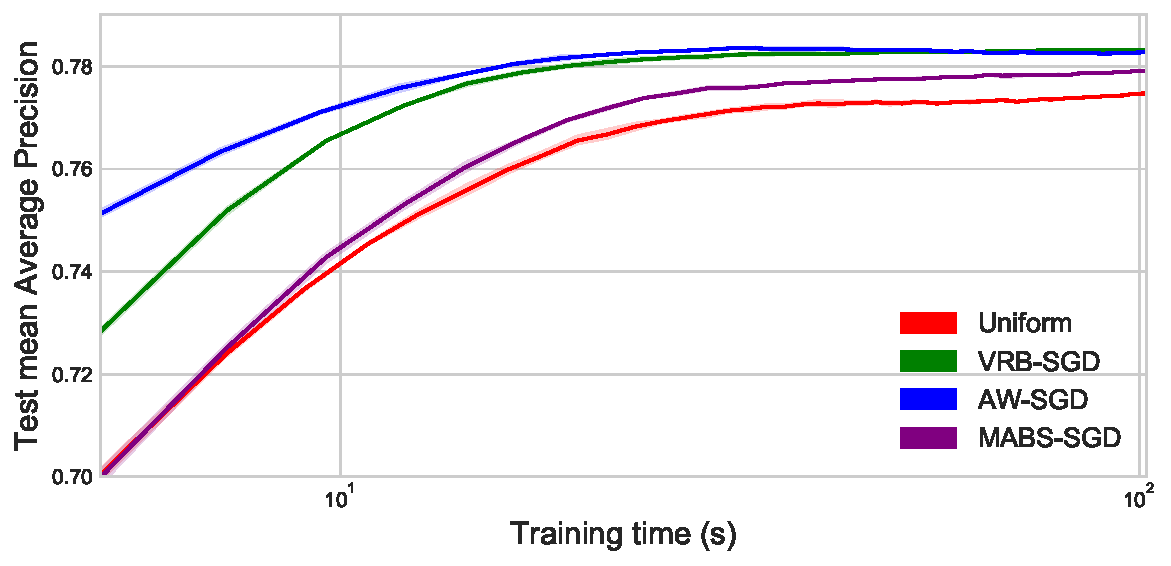
\includegraphics[width=\linewidth]{figures/voc-result.pdf}
      \caption{Mean Average Precisions on the test part of VOC 2007.}
      \label{fig:voc-results}
\end{minipage}%
\quad
\begin{minipage}{.48\textwidth}
  \centering
  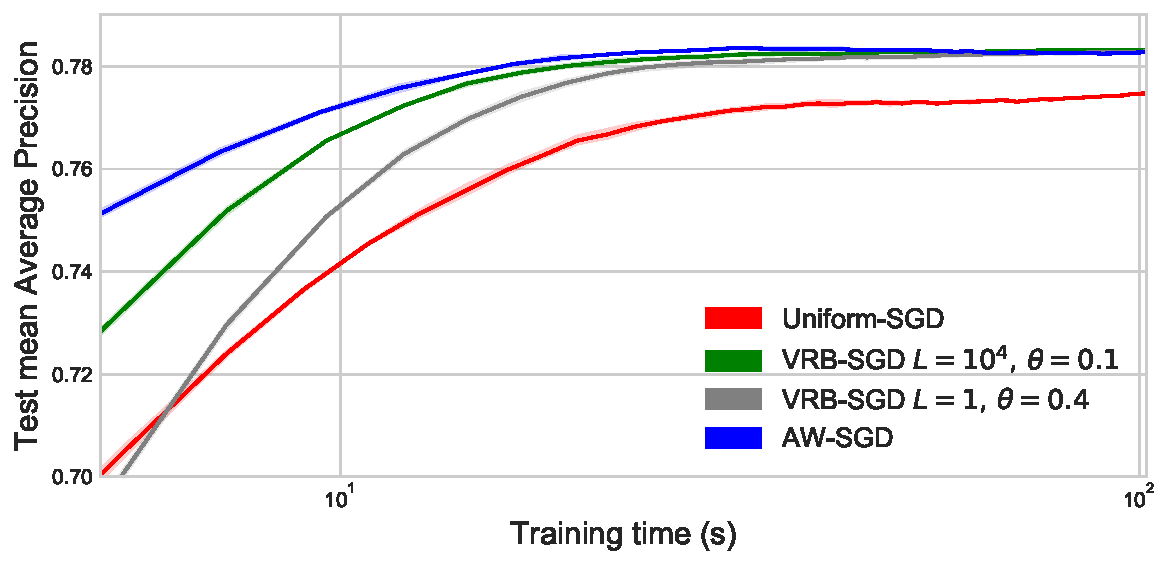
\includegraphics[width=\linewidth]{figures/voc-result-2.pdf}
      \caption{The effect of different hyperparameters on VRB. }
      \label{fig:voc-results-2}
\label{fig:test}
\end{minipage}%
\end{figure}

        
The hyperparameters of the methods are chosen based on cross-validation on the validation portion of the dataset. The results can be seen in Figure \ref{fig:voc-results}, where the shaded areas represent confidence $95\%$ intervals over 10 runs. The best performing method is AW, but its disadvantage compared to the bandit algorithms is that it requires choosing a family of sampling distributions, which usually incorporates prior knowledge, and calculating the derivative of the log-density. VRB and AW both outperform uniform subsampling with respect to the training time.  VRB performs similarly to AW at convergence, and speeds up training 10 times compared to uniform sampling, by attaining a certain score level 10 times faster. We have also experimented with the variance reduction method of \cite{pmlr-v70-namkoong17a}, but it did not outperform uniform sampling significantly. Since cross-validation is costly, in Figure \ref{fig:voc-results-2} we show the effect of the hyperparameters of our method. More specifically, we compare the performance of VRB with misspecified regularizer $L=1$ to the best $L=10^8$ chosen by cross-validation, and we compensate by using higher mixing coefficient $\theta=0.4$. The fact that only the early-stage performance is affected is a sign of method's robustness against regularizer misspecification.

We also measure the regret incurred both by the full information and VRB samplers, and show the results in Figure \ref{fig:regret}. For a fair comparison, we choose an \emph{oblivious} adversary that generates the loss sequences by performing the same optimization process as described above on a subset of 1000 data points from VOC 2007, with uniform sampling. For VRB, we report the average regret over 10 runs. 
\begin{figure}[h]

		\centering
		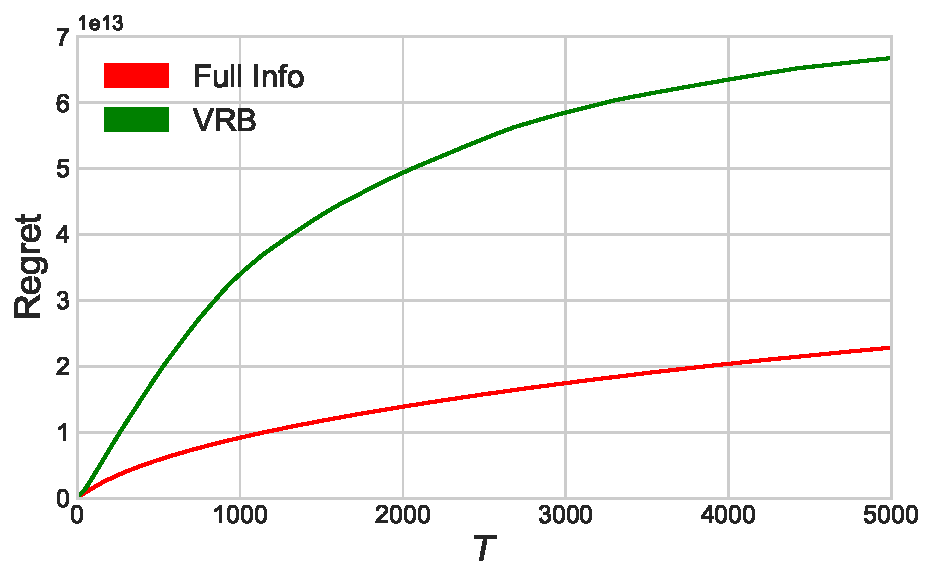
\includegraphics[width=0.5\linewidth]{figures/regret.pdf}
		\caption{Regret incurred by the full info and VRB.}
		\label{fig:regret}
\end{figure}


\subsection{$k$-Means}

In this experiment, we show that in some applications it is beneficial to work with per-sample upper bound estimates $L_i$ instead of a single global bound. As an illustrative example, we choose mini-batch $k$-Means clustering \citep{sculley2010web}. This is a slight deviation from the presented theory, since we sample multiple points for the batch and update the sampler only  once, upon observing the loss for the batch. 

In the case of $k$-Means, the parameters consist of the coordinates of the $k$ centers \linebreak $Q=\{q_1, q_2, \dots, q_k\}$. As the cost function for a point $x_i \in \{x_1, x_2, \dots, x_n \}$ is the  squared Euclidean distance to the closest center, the loss received by VRB  is the norm of the gradient  \linebreak $\min _{q \in Q } 2 \cdot || x_i - q||_2$. This lends itself to a natural estimation of $L_i$:
choose a point $u$ randomly from the dataset and define $L_i=4 \cdot || x_i - u||^2_2$. For this experiment, we set $\theta=0.5$.

We solve mini-batch $k$-Means  for $k=100$ and batch size $b=100$ with uniform sampling and VRB. The initial centers are chosen with $k$-Means++ \citep{arthur2007k} from a random subsample of 1000 points from the training data and they are shared between the methods. We generate 10 different sets of initial centers and run both algorithms 10 times on each set of centers, with different random seeds for the samplers.  We train the algorithm on $80 \%$ of the data, and measure the cost of the $20 \%$ test portion for the following datasets:
\vspace{-2mm}
\begin{itemize}
\setlength\itemsep{0.2em}
  \item \texttt{CSN} \citep{faulkner2011next} --- cellphone accelerometer with 80,000 observations and 17 features,
 \item \texttt{KDD} \citep{kddcup2004} --- data set used for Protein Homology Prediction KDD
    competition  containing 145,751 observations with 74 features,
    \item \texttt{MNIST} \citep{lecun1998gradient} --- 70,000 low resolution images of handwritten
    characters transformed using PCA with whitening and retaining 10 dimensions.  
\end{itemize}

\begin{figure}[h]
      \centering
      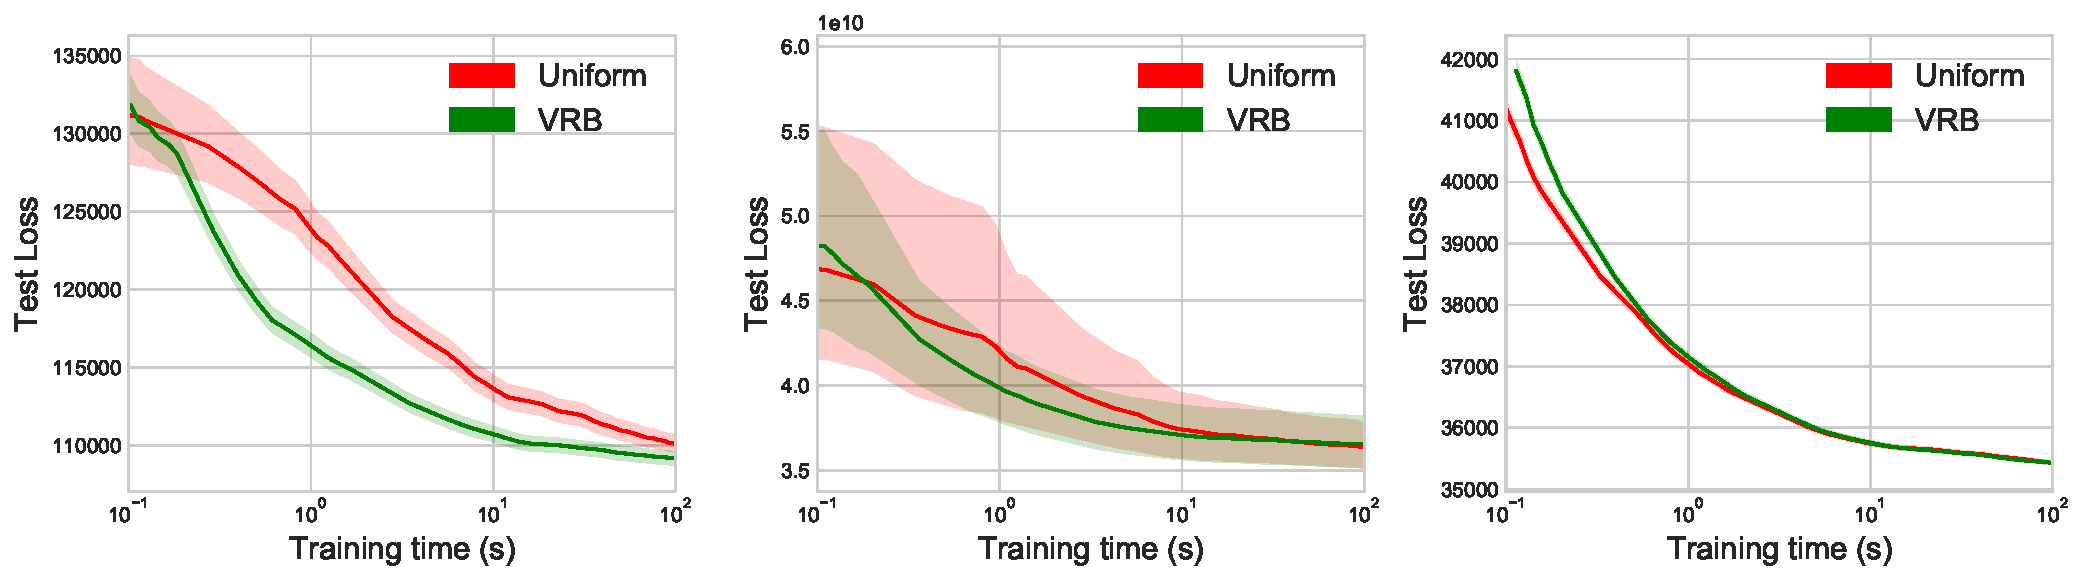
\includegraphics[width=\linewidth]{figures/kmeans.pdf}
      \caption{The evolution of the loss of $k$-Means on the test set. The shaded areas represent $95\%$ confidence intervals over 100 runs.}
      \label{fig:kmeans-results}
        \end{figure}
        
The evolution of the cost function on the test set with respect to the elapsed training time is shown in Figure \ref{fig:kmeans-results}. The chosen datasets illustrate three observed behaviors of our algorithm. In the case of \texttt{CSN}, our method significantly outperforms uniform subsampling. In the case of \texttt{KDD}, the advantage of our method can be seen in the reduced variance of the cost over multiple runs, whereas on \texttt{MNIST} we observe no advantage.
This behavior is highly dependent on intrinsic dataset characteristics: for \texttt{MNIST}, we note that the entropy of the best-in-hindsight sampling distribution is close the entropy of the uniform distribution. We have also compared VRB with the bandit algorithms mentioned in the previous section. Since mini-batch $k$-Means converges in 1-2 epochs, these methods with  uniform initialization do not outperform uniform subsampling significantly. Thus, for this setting, careful initialization is necessary, which is naturally supported by our method.

